
\setlength{\parskip}{0pt} % Espaciado compacto
\setlength{\parindent}{0em}

% Configuración del entorno "Solución"
\theoremstyle{nonumberplain}
\theoremheaderfont{\itshape}
\theorembodyfont{\upshape}
\theoremseparator{.}
\theoremsymbol{\ensuremath{\square}}
\newtheorem{solucion}{Solución}



\textbf{Problema:} Maximizar \( U(x, y) \) sujeta a \( 2x + y = 30 \). \\

\begin{solucion}
La función de Lagrange \( \mathcal{L} \) se define como:
\[
\mathcal{L}(x, y, \lambda) = U(x, y) - \lambda (2x + y - 30)
\]
Donde \( \lambda \) es el multiplicador de Lagrange. Calculamos las derivadas parciales:
\[
\frac{\partial \mathcal{L}}{\partial x} = y + 2 - 2\lambda = 0 \quad (1), \quad 
\frac{\partial \mathcal{L}}{\partial y} = x - \lambda = 0 \quad (2), \quad 
\frac{\partial \mathcal{L}}{\partial \lambda} = 2x + y - 30 = 0 \quad (3)
\]
De (2): \( \lambda = x \). Sustituyendo en (1):
\[
y + 2 - 2x = 0 \implies y = 2x - 2 \quad (4)
\]
Sustituyendo \( y = 2x - 2 \) en (3):
\[
2x + (2x - 2) = 30 \implies 4x - 2 = 30 \implies x = 8
\]
Con \( x = 8 \), en (4): \( y = 2(8) - 2 = 14 \).

Sustituyendo \( x = 8 \), \( y = 14 \) en \( U(x, y) = xy + 2x \):
\[
U(8, 14) = 8 \cdot 14 + 2 \cdot 8 = 112 + 16 = 128
\]
\(\therefore\) El valor máximo de la utilidad es \( 128 \), alcanzado en \( (x_0, y_0) = (8, 14) \). \\

\begin{figure}[h]
    \centering
    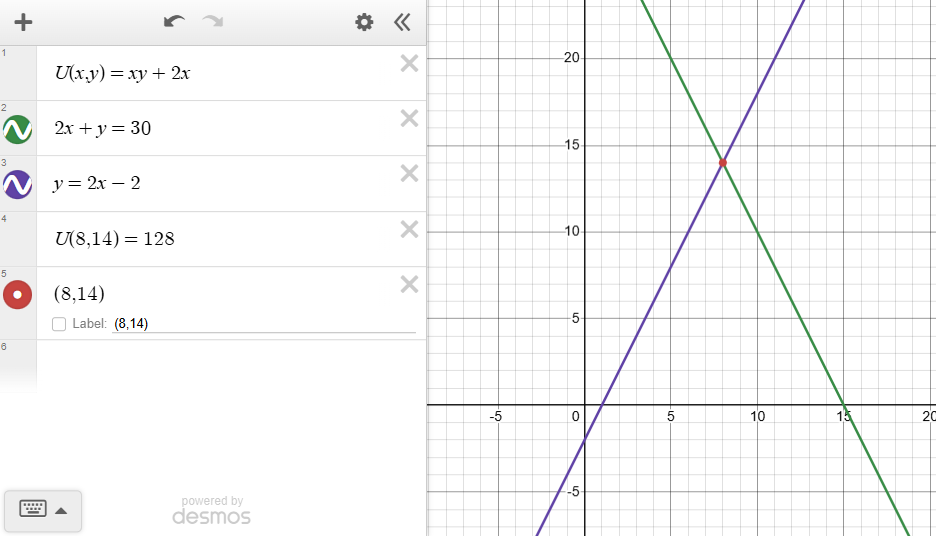
\includegraphics[width=0.55\linewidth]{Graphic i.png}
    \caption{Gráfica de \( U(x, y) \) y la restricción \( 2x + y = 30 \).}
\end{figure}

\end{solucion}


